\documentclass[conference]{IEEEtran}
\IEEEoverridecommandlockouts
% The preceding line is only needed to identify funding in the first footnote. If that is unneeded, please comment it out.
\usepackage[utf8]{inputenc}
\usepackage[english]{babel}
\usepackage{cite}
\usepackage{amsmath,amssymb,amsfonts}
\usepackage{physics}
\usepackage{dsfont}
\usepackage{algorithmic}
\usepackage{graphicx}
\usepackage{subcaption}
\usepackage{array}
\usepackage{float}
\usepackage{lipsum}
\usepackage{textcomp}
\usepackage{xcolor}
\usepackage{diagbox}

\usepackage[hidelinks]{hyperref}
\def\BibTeX{{\rm B\kern-.05em{\sc i\kern-.025em b}\kern-.08em
    T\kern-.1667em\lower.7ex\hbox{E}\kern-.125emX}}
\begin{document}

\title{Simulation of ARMAX model for \\}

\author{\IEEEauthorblockN{Juan S. C\'ardenas R.}
\IEEEauthorblockA{\textit{Student} \\
\textit{Universidad EAFIT}\\
Medell\'in, Colombia\\
jscardenar@eafit.edu.co}
\and
\IEEEauthorblockN{David Plazas E.}
\IEEEauthorblockA{\textit{Student} \\
\textit{Universidad EAFIT}\\
Medell\'in, Colombia \\
dplazas@eafit.edu.co}
}

\maketitle

\begin{abstract}

\end{abstract}

\begin{IEEEkeywords}

\end{IEEEkeywords}
\section{Introduction}
The system in study was proposed by O.E. R\"ossler  in 1976, as a simplified model with shape and behavior similar to spirals in Lorenz system, which was not fully understood at the time due to the techniques known to study oscillators were not applicable to Lorenz model \cite{rossler1976equation}. The R\"ossler equations are:

\begin{equation}
	\begin{array}{ll}
            \dot{x}&=-y-z\\
            \dot{y}&=x+ay\\
            \dot{z}&=b+z\left(x-c\right)
    \end{array}
\end{equation}

Although R\"ossler affirmed that the system did not have immediate physical interpretation \cite{rossler1976equation}, nowadays some applications can be found using the model as a mechanism and not as an abstraction of a physical system. The model presented has been used as a tool for image cryptography as it was shown by Mandal \textit{et al.} in  \cite{mandal2014symmetric}; in further work, Laiphrakpam and Khumanthem proposed improvements to Mandal's algorithm, as it is shown in \cite{laiphrakpam2017cryptanalysis}. On the other hand, coupled R\"ossler system with different inputs have been used to measure the correlation of time series, as Weule \textit{et al.} showed in \cite{weule1998detection}.

In order to bring the system to the real world, R\"ossler equations can be represented by a circuit, as Canals \textit{et al.} show in \cite{canals2014random}. The proposed circuit is shown in Fig. \ref{fig:circuito} and can be translated to 
\begin{equation}
	\begin{array}{ll}
            RC\dot{x}&=-y-z\\
            RC\dot{y}&=x+ay\\
            RC\dot{z}&=b+z\left(x-c\right)
    \end{array}\quad\quad\begin{array}{ll}
            a &= \dfrac{100k\Omega}{R_a}\vspace{2.5mm}\\
            b &= V_{cc}\dfrac{100k\Omega}{R_b}\vspace{2.5mm}\\
            c &= \dfrac{100k\Omega}{R_c}
    \end{array}\label{eq:circ}
\end{equation}
In \cite{canals2014random} they use this circuit to generate true random numbers using the output of the voltage of the node $z$. The nodes $x$ and $y$ have a fixed frequency of oscillation if the other variable is set to 0, since their rate of change are linear. In contrast, $z$ induces chaos to the circuit, due to its nonlinear behavior. In this manner, this variable was selected to be the output as its chaotic behavior is useful to generate random numbers \cite{canals2014random}.

In previous work \cite{JS_PL}, it was found that the Rössler system is stable for large input values. Based on this, it will be attempted to analyze this system as a linear model.

In this work, the question ``which linear model can successfully represent the Rössler circuit for certain input and parameters?''. It is difficult to give a hypothetical model without prior linear analysis, although it is believed that this model to be found will represent the system behavior, at least, in stationary state.

In order to achieve this, this work will begin linearizing the system in an equilibrium point, comparing the time response for both systems, close and far away from the operation point. Then, the respective continuous and discrete transfer function will be obtained and compared with the continuous linear model. It will be attempted to reduce the model's order using both analytic and software methods and compare this models with the linearized Rössler system; on the other hand, an stability analysis will be performed, using Ruth-Hurwitz criteria and root locus method. Finally a frequency response analysis will be performed using Bode diagrams of the original linearized model and the reduced ones; based on the Bode diagram for the linearized system, the closed-loop stability will be determined using phase and gain margins.

In section \ref{sec:meth}, the dynamic system used and some theory required to make the linear analysis of the Rössler system can be found. In section \ref{sec:results}, the results of every procedure are presented and applied to the Rössler system. In section \ref{sec:resultAn}, the analysis of the obtained results and their justification is made. Finally, the conclusions are presented in section \ref{sec:conc}.

%PREGUNTA INV; OBJETIVOS; TABLA CONTENIDOS, Etc.
\begin{figure*}
    \centering
    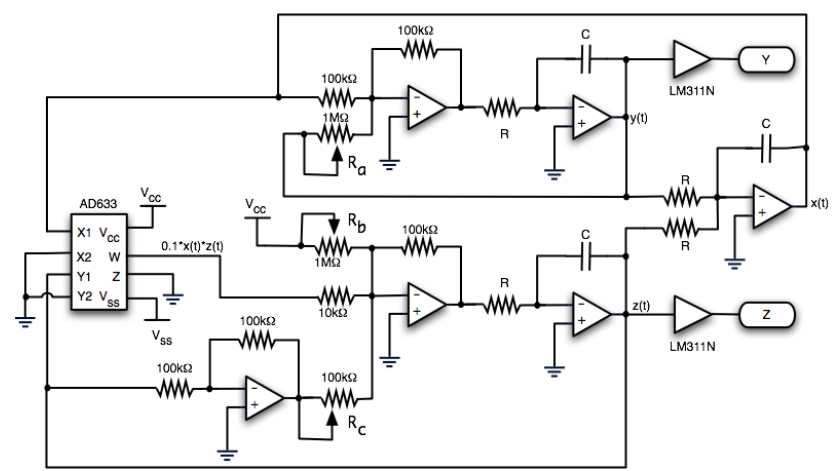
\includegraphics[scale=0.325]{figs/Circuito.png}
    \caption{R\"ossler circuit representation \cite{canals2014random}.}
    \label{fig:circuito}
\end{figure*}
\section{Methods}\label{sec:meth}
\subsection{Dynamic System}
In the circuit presented, according to Canals \textit{et al.} \cite{canals2014random}, the variables $x$, $y$ and $z$ represent the voltages through the nodes shown in Fig. \ref{fig:circuito}. The $RC$ parameter defines the system's time (in seconds), the supplied voltages are $V_{cc}=15V$ and $V_{ss}=-15V$; $R_a$, $R_b$ y $R_c$ are resistors in $k\Omega$ used to calculate the system's original parameters, as shown in (\ref{eq:circ}).

The circuit can be represented through a dynamic equation, as follows:
\begin{equation}
\begin{cases}
	\dot{x_1}=\dfrac{1}{RC}\left(-x_2-x_3\right)&\vspace{2mm}\\\vspace{2mm}
	\dot{x_2}=\dfrac{1}{RC}\left(x_1+\dfrac{100k\Omega}{R_a}x_2\right)&\\
	\dot{x_3}=\dfrac{1}{RC}\left[\left(V_{cc0}+u\left(t\right)\right)\dfrac{100k\Omega}{R_b}+x_3\left(x_1-\dfrac{100k\Omega}{R_c}\right)\right]&\\
	y = x_3
\end{cases}
\label{eq:state}
\end{equation}
where $y$ is the output and $u$ the input; note that the parameter $V_{cc}$ was selected as input, based on equation (\ref{eq:circ}), thus we select an initial value $V_{cc0}$ and add the input $u\left(t\right)$ in Volts. For the rest of this document, the state variable $x_3$ can sometimes be referred as $y$, since it has been chosen as the output.

\subsection{Simulation Diagram}
Using equation system (\ref{eq:state}), a simulation diagram was constructed using \textit{Simulink}, as Fig. \ref{fig:simulink} shows.
\begin{figure}
    \centering
    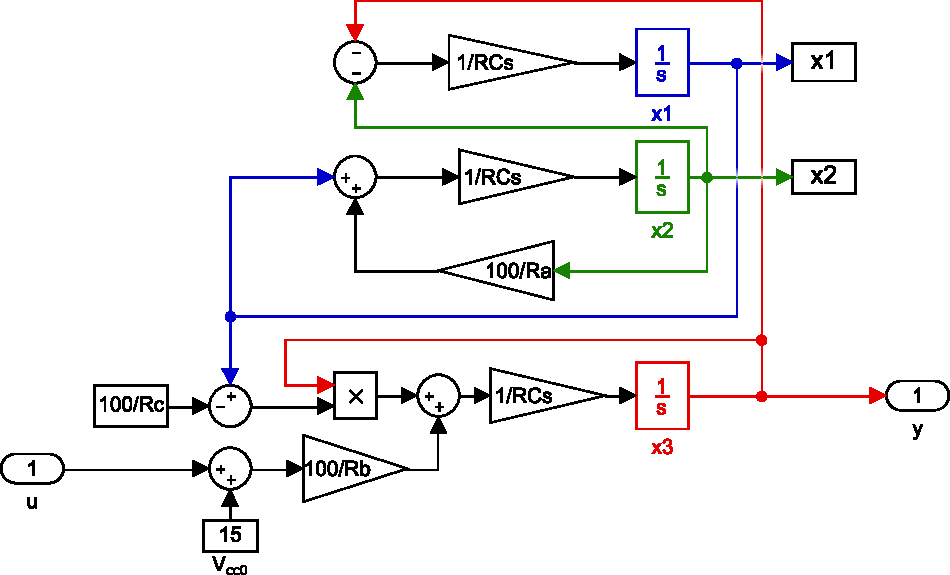
\includegraphics[scale=0.55]{figs/simulink.pdf}
    \caption{Simulation diagram for R\"ossler system.}
    \label{fig:simulink}
\end{figure}

\subsection{Linearity Curve}
The linearity curve is a tool that helps determine the range where the linear system can provide a suitable approximation to the stable nonlinear system. The linearity curve is obtained by simulating an stable system and registering the final value (stationary state) for a constant input, then the input is increased in a constant factor and then simulated until a new final value is found and so forth.

For the system in study, the following simulation diagram (Fig. \ref{fig:linearitySimulink}) was constructed, using \textit{Simulink}, in order to obtain the desired curve. As this figure shows, both systems are simulated with the same input. This one begins with a clock that should represent a continuous ``ramp'' over time, which is first scaled by a factor of $2/10$ and then passes through a Zero-Order-Hold (ZOH). This ZOH ensures that the continuous ``ramp'' is transformed into a discrete one, i.e. a ``staircase'' input since the signal is retained with a sampling time of $T=100s$. This means that both systems are simulated for $100s$ with a \textbf{constant} input. After this, the ZOH passes a new constant signal, where each iteration of the ZOH increases the input by $20V$ (this explains why it is scaled by $2/10$). Note that the initial input value $1000V$ has been included in the nonlinear simulation diagram, as Fig. \ref{fig:simulink} shows.
\begin{figure}[H]
    \centering
    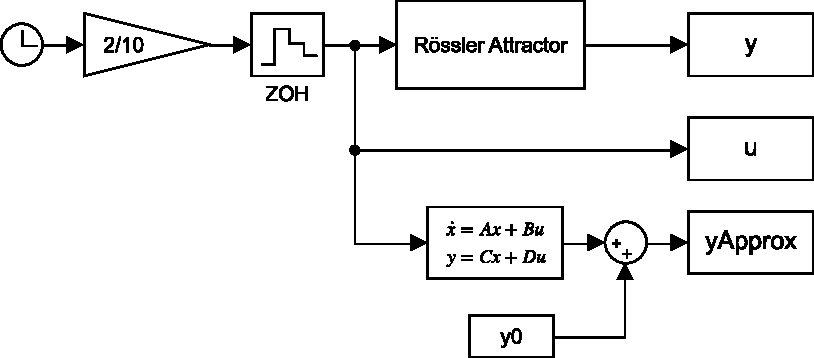
\includegraphics[scale=0.55]{figs/linearCurveSimulink.pdf}
    \caption{Simulation diagram for linearity curve.}
    \label{fig:linearitySimulink}
\end{figure}

\subsection{Linearization}
In order to linearize the system in study, the classical procedure will be performed. For more detailed notes on this method, see \cite[pp. 21-27]{antsaklis2007linear}. Given a nonlinear dynamic system
\begin{equation}
\begin{split}
    \mathbf{\dot{x}} =& f(\mathbf{x},\mathbf{u})\\
    \mathbf{y}=&g(\mathbf{x},\mathbf{u})
\end{split}
\end{equation}
We can obtain a linearization of this system around an operation point $(\mathbf{x_0},\mathbf{u_0})$, in the form
\begin{equation}\label{eq:stateLinear}
\begin{split}
    \Delta\mathbf{\dot{x}} =& \mathbf{A} \Delta\mathbf{x}+\mathbf{B}\Delta\mathbf{u}\\
    \Delta\mathbf{y}=&\mathbf{C}\Delta\mathbf{x}+\mathbf{D}\Delta\mathbf{u}
\end{split}
\end{equation}
Where $\Delta \mathbf{x}=\mathbf{x}-\mathbf{x_0}$, $\Delta \mathbf{u}=\mathbf{u}-\mathbf{u_0}$, $\Delta \mathbf{y}=\mathbf{y}-\mathbf{y_0}$; and $\mathbf{A}$, $\mathbf{B}$, $\mathbf{C}$ and $\mathbf{D}$ are Jacobians of the functions $f$ and $g$ as follows
\begin{equation}
\begin{split}
    \mathbf{A}=\dfrac{\partial f}{\partial\mathbf{x}}(\mathbf{x_0},\mathbf{u_0})&\qquad \mathbf{B}=\dfrac{\partial f}{\partial\mathbf{u}}(\mathbf{x_0},\mathbf{u_0})\\
    \mathbf{C}=\dfrac{\partial g}{\partial\mathbf{x}}(\mathbf{y_0},\mathbf{u_0})&\qquad \mathbf{D}=\dfrac{\partial g}{\partial\mathbf{u}}(\mathbf{y_0},\mathbf{u_0})
\end{split}
\end{equation}
This procedure can be also performed using \textit{Matlab}, through the command \texttt{linmod} with the following syntax: \texttt{[$\mathbf{A}$,$\mathbf{B}$,$\mathbf{C}$,$\mathbf{D}$] = linmod(\textit{sys},$\mathbf{x}_0$,$\mathbf{u}_0$)}, where \texttt{\textit{sys}} is a \textit{Simulink} model, and $(\mathbf{x}_0,\mathbf{u}_0)$ is the operation point.

\subsection{Linear and Nonlinear systems comparison}
As it has been already depicted, the linearization of a nonlinear model is given in $\Delta$-variables; in order to compare properly the output of a nonlinear system and its linearization, the scheme shown in Fig. \ref{fig:howto} can be used. Note that, for the linear system, is required to subtract the initial input $\mathbf{u_0}$ to obtain $\Delta\mathbf{u}$, and the output is given as $\Delta\mathbf{y}$, then the initial value $\mathbf{y_0}$ is added to obtain the standard output $\mathbf{y}(t)$
\begin{figure}[H]
    \centering
    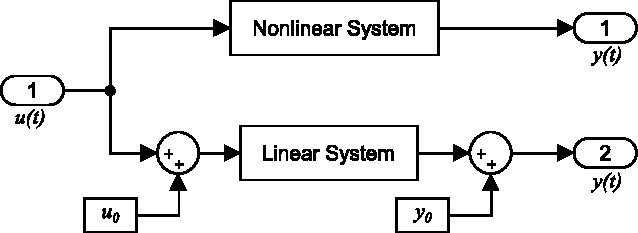
\includegraphics[scale=0.6]{figs/howtoLinearNonlinear.pdf}
    \caption{Diagram for comparing a nonlinear system with its linearization.}
    \label{fig:howto}
\end{figure}

\subsection{Transfer Function}\label{sec:tf}
The transfer function is a tool to represent a linear system with null initial conditions. For a single-input single-output (SISO) system, it is defined as the relation between the Laplace transform ($\mathcal{L}$) of the output and the Laplace transform of the input, as follows:
\begin{equation}
    G(s)=\dfrac{Y(s)}{U(s)}
\end{equation}
Where $Y(s)=\mathcal{L}\{y(t)\}$, $U(s)=\mathcal{L}\{u(t)\}$. For a discrete system, it would be worked with the $\mathcal{Z}$ transform. If the system is in a state-space representation, as in equation (\ref{eq:stateLinear}), the transfer function can be also obtained with
\begin{equation}\label{eq:ss2tf}
    G(s)=\mathbf{C}(s\mathbf{I}-\mathbf{A})^{-1}\mathbf{B}+\mathbf{D}
\end{equation}

And, finally, this can be achieved using \textit{Matlab}, using the command \texttt{tf(\textit{LinSys})}, where \texttt{\textit{LinSys}} is a linear system object (can be created with the command \texttt{ss($\mathbf{A}$,$\mathbf{B}$,$\mathbf{C}$,$\mathbf{D}$)}).

\subsection{Sampling Time}\label{sec:sampling}
The sampling time is a number that determines how often a continuous signal will be sampled in order to obtain a discrete signal.

In this work, the sample time was originally selected empirically, based on simulation: it was chosen such that the signal is sampled correctly (keeping oscillation period and most transitory behavior) and such that it can be easily evidenced the ``retained'' signal.

From a theoretical perspective, the sampling time can be obtained from the growth time ($T_r$) of the system in study. The growth time is defined at the time that the system takes to reach $90\%$ of stationary state from the respective $10\%$, and then apply the following criterion:
\begin{equation}
    \dfrac{T_r}{10}<T<\dfrac{T_r}{2}
\end{equation}
It is important to mention that the sample time selection is a non-trivial procedure, since a bad selection of the sample time can lead to undesired phenomena like the aliasing; for more information regarding the sample theorem and aliasing, refer to \cite[pp. 34-54]{diniz2010digital}. In this work, both methods are performed.

\subsection{Discretization of Transfer Functions}\label{sec:c2d}
Given a continuous transfer function $G(s)$, the discrete transfer function is obtained through the following expression:
\begin{equation}
    G(z)=(1-z^{-1})\mathcal{Z}\left\{\mathcal{L}^{-1}\left\{\dfrac{G(s)}{s}\right\}_{t\rightarrow kT}\right\}
\end{equation}
Where $T$ is a predefined sampling time for the discretization. This procedure can also be carried out using \textit{Matlab} with the command \texttt{c2d(\textit{transfer},T)} and, in this case, \texttt{\textit{transfer}} is a continuous transfer function.

\subsection{Ponderation Sequence}\label{sec:ponderationSequence}
The transfer function can be used to obtain a sequence of numbers that, given an input, the respective system output can be acquired. This numbers, in a continuous system, are infinite; thus, this sequence is often calculated for the discrete case.

Let $G(z)$ a discrete transfer function. The discrete ponderation sequence is found from the inverse $\mathcal{Z}$ transform of this transfer function:
\begin{equation}
    g(k)=\mathcal{Z}^{-1}\{G(z)\}
\end{equation}
And the output can be calculated with the following procedure:
\begin{equation}
    \begin{split}
        G(z)&=\dfrac{Y(z)}{U(z)}\\
        Y(z)&=G(z)U(z)\\
        \mathcal{Z}^{-1}\left\{Y(z)\right\}&=\mathcal{Z}^{-1}\left\{G(z)U(z)\right\}\\
        y(k)&=g(k)*u(k)
    \end{split}
\end{equation}
Where $*$ represent the convolution product, in this case, discrete.


\subsection{Order Reduction}\label{sec:reduct}
In order to reduce the system order, two straight-forward methods are often considered; this methods do not require formal procedures.

The first method is to cancel out stable zeros and poles that are close enough to each other and add a gain to assure that the stationary state for both systems is equal. The second method is to cancel out stable poles that are far enough from the dominant pole (at least 10 times the dominant pole) and, as the previous method, add a gain to compensate for the reduction.

On the other hand, in order to reduce the system order with more formal methods, \textit{Matlab} has the command \texttt{balred(\textit{Linear},\textit{order})}, where \texttt{\textit{Linear}} is an state-space model \textbf{or} a transfer function, and \texttt{\textit{order}} is the desired order after the reduction.

\textbf{2nd order approximation:\\} This method is a slightly more empirical/experimental approach. This method is based on the general formula for 2nd order transfer functions:
\begin{equation}
    G(s)=\dfrac{k\omega^2_0e^{-s\tau}}{s^2+2\zeta\omega_0s+\omega_0^2}
\end{equation}
Where $\omega_0$ is the natural frequency of the system, $\zeta$ is the damping, $k$ is the gain and $\tau$ is the delay. An example is shown in Fig. \ref{fig:example2ndOrder}.
\begin{figure}[H]
    \centering
    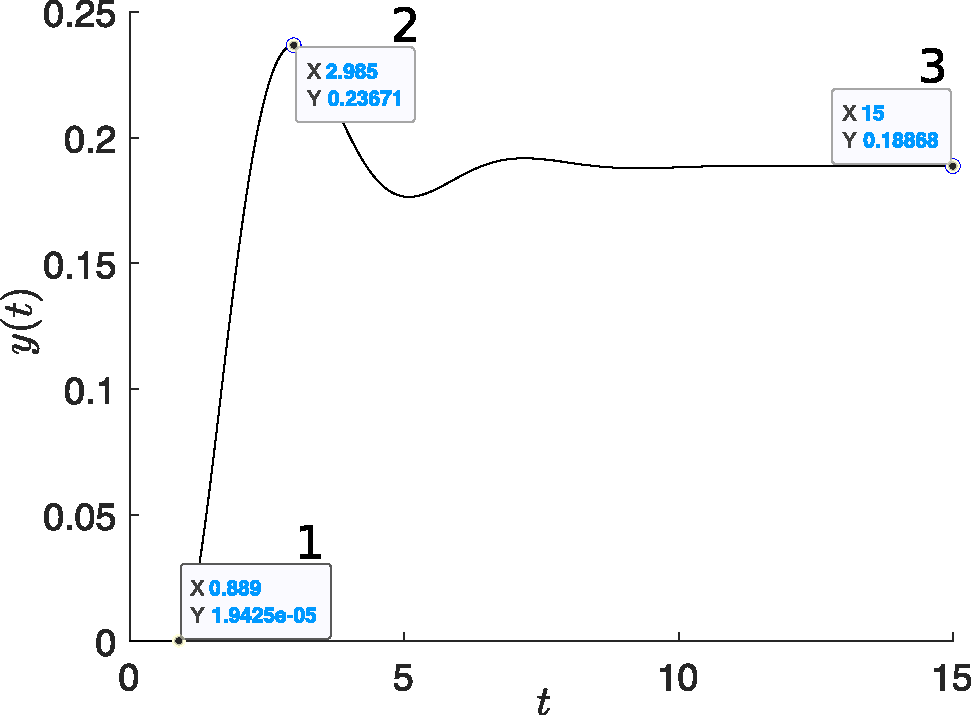
\includegraphics[scale=0.4]{figs/sis2ndOrder.pdf}
    \caption{Second order system.}
    \label{fig:example2ndOrder}
\end{figure}
In order to calculate the parameters, points 1, 2 and 3 are required. The first point gives information about the delay $\tau$, the second has information about the peak time $t_p$ and magnitude $y_p$. Finally, the last one shows the final value $y_{ss}$ (stationary state) and is needed to calculate the gain.

The following expression is used to calculate $\zeta$:
\begin{equation}
    \zeta=\dfrac{1}{\sqrt{1+\left(\dfrac{\pi}{\ln Mp}\right)^2}}
\end{equation}
Where
\begin{equation}
    Mp=\dfrac{y_p-y_{ss}}{y_{ss}}
\end{equation}
is the maximum overshoot; and through the following equation, $\omega_0$ is obtained:
\begin{equation}
    \omega_0=\dfrac{\pi}{t_p\sqrt{1-\zeta^2}}
\end{equation}

\subsection{Stability}
The following methods can only be applied to linear systems. For stability of nonlinear systems see reference \cite[Ch. 13]{dahleh2004lectures}, for Lyapunov stability.
\subsubsection{Poles Calculation}
The simplest way of knowing whether a linear system is stable is calculating all the poles $\lambda_i$ and checking if $\Re(\lambda_i)<0$. In \textit{Matlab}, the poles can be calculated directly from the state-space model or transfer function with the command \texttt{pole(\textit{Linear})}.

\subsubsection{Bounded-Input Bounded-Output Criterion (BIBO)}
Another way to determine if a linear system is stable is through the BIBO criterion \cite[Pag. 170]{antsaklis2007linear}: a bounded input (e.g. bounded waves, step, impulse train, etc.) generates a bounded output. It is important to highlight that this criterion does not necessarily imply that for every bounded input, the output will be bounded, but at least, for sine inputs. Another note is that this method is specially important when poles are exclusively imaginary ($\Re(\lambda_i)=0$).

\subsubsection{Routh-Hurwitz Method}
The Routh-Hurwitz method works with the characteristic polynomial of a linear system, that can be obtained from the denominator of the transfer function or with $P(s)=|s\mathbf{I}-\mathbf{A}|=0$.

Consider the general case:
\begin{equation}
    P(s)=\sum_{j=0}^na_js^{n-j}\quad a_0\neq0
\end{equation}
\textbf{Necessary Conditions:}
\begin{itemize}
    \item $(\forall j)(a_j>0)$
\end{itemize}
\textbf{Sufficient Conditions:}
\begin{itemize}
    \item The first column of the Routh-Hurwitz array is non-negative.
\end{itemize}

For a more detailed explanation of the Routh-Hurwitz array, refer to \cite[pp. 212-214]{ogata2010modern}. In \textit{Matlab}, an implementation has been developed and can be found in \cite{RHCaliche}.

\subsection{Root Locus}\label{sec:root_locus}
The root locus is a plot of how the roots of a polynomial change for a parameter $k>0$. It uses a closed-loop transfer function with a gain $k$ that is equivalent to this polynomial.

Given a polynomial with the parameter $k$ in one or more coefficients of the polynomial, it can always be expressed as 
\begin{equation}
    1+k\dfrac{N(s)}{D(s)}=0
\end{equation}
Note that this can be interpreted as a denominator of a closed-loop transfer function. Thus, the associated plant is 
\begin{equation}
    G(s)=\dfrac{N(s)}{D(s)}
\end{equation}

The root locus starts ($k=0$) in the poles of $G(s)$ and finishes ($k\rightarrow\infty$) in the finite and infinite zeros of $G(s)$. The root locus is useful to determine ranges of $k$ where the system associated with the characteristic polynomial $P(s)$ is stable. This procedure can also be used to determine the infinite zeros of a transfer function. The root locus can be obtained as well using \textit{Matlab} using \texttt{rlocus(\textit{Linear})}, where \texttt{\textit{Linear}} is a state-space model or a transfer function.

\subsection{Bode Diagram}\label{sec:bode}
The Bode diagram is a tool to analyze the frequency response. The frequency response is useful to analyze the system output when the input is a sine wave, since the output in stationary state will be another sine wave with equal frequency and different amplitude and phase.

The bode diagram is composed of two plots in logarithmic scale, since it is often desired to analyzed the frequency response for a wide spectrum of frequencies: one for the relative amplitude and another one for the phase of the output (in stationary state). For the amplitude, it is given in decibels (dB) and for the phase, it is given in degrees.

Suppose the input is
\begin{equation}
    u(t)=A\sin(\omega t)
\end{equation}
And the output in stationary state
\begin{equation}
    y_{ss}(t)=B\sin(\omega t+\phi)
\end{equation}
It can be proved (see \cite[pp. 399-400]{ogata2010modern}) that \[B=A|G(i\omega)|\]\[\phi=\arctan\left(\dfrac{\Im[G(i\omega)]}{\Re[G(i\omega)]}\right)\] And the amplitude in decibels is defined as 
\begin{equation}
    |G(i\omega)|\text{dB}=20\log_{10}\left(\dfrac{B}{A}\right)
\end{equation}
The Bode diagram is useful for several reasons. In first place, it can be used to determine the regions where the system intensifies or reduces the input amplitude. On the other hand, it can be used to determine the ranges of gain and delay where the closed-loop system is stable. Lastly, it can help determine whether the system in study is a minimum phase system.

The bode diagram can be obtained using \textit{Matlab} through the command \texttt{bode(\textit{Linear})}, where \texttt{\textit{Linear}} is a transfer function or a linear state-space model.

As it was previously mentioned, the Bode diagram can be used to determine closed-loop stability, using the phase and gain margins. For a more detailed explanation regarding the phase and gain margins see \cite[pp. 464-468]{ogata2010modern}. With \textit{Matlab}, the margins can be calculated with the command \texttt{allmargin(\textit{Linear})}, where Linear is a state-space model or a transfer function.

\section{Problem Formulation}\label{sec:probForm}
As previously mentioned, the output of the PV system is an stochastic process. The standard approach to forecasting the behavior of this system has been modelled using ARIMA models, using only information of the past of the same system, but it does not take into consideration the external environmental factors that may affect the power output \cite{li2014armax}; as for the problem of this particular work, the main objective is to simulate the ARMAX model proposed in \cite{li2014armax} with different noise distributions, particularly with outlier behavior and show that it is not always adequate to assume normality of some random processes.

\section{Theoretical Approach}\label{sec:theo}
\subsection{General ARMAX model}

As previously mentioned, this work uses an ARMAX model presented in the literature; hereby, let the general ARMAX model be presented:
\begin{equation}
    z_{t+1}=\sum_{i=0}^{h_1}a_iz_{t-i}+\sum_{i=0}^{h_2}b_iu_{t-i}+\sum_{i=0}^{h_3}c_i\xi_{t-i}
\end{equation}
for $t=0,1,2,\ldots$, and $u_k$ are external inputs and $\xi_k$ are random noises. In this particular case, the model obtained in \cite{li2014armax} is:
\begin{equation}
\begin{aligned} z_{t}=& 237.565+0.426z_{t-1}+\xi_{t}-0.153 \xi_{t-1}+8.9087u_{1, t} \\ &-1.557 u_{7, t}+31.919 u_{8, t}-2.045u_{9, t}
\end{aligned}
\end{equation}
where $z_t$ is the power output of the PV grid in Watts (W); $u_{1,t}$ is the daily average temperature, $u_{7,t}$ is the precipitation amount, $u_{8,t}$ is the insolation duration and $u_{9,t}$ is the humidity.
\section{}

\section{Numerical Aspects}\label{sec:numAsp}
In this particular case, the model obtained in \cite{li2014armax} is:
\begin{equation}
\begin{aligned} z_{t}=& 237.565+0.426z_{t-1}+\xi_{t}-0.153 \xi_{t-1}+8.9087u_{1, t} \\ &-1.557 u_{7, t}+31.919 u_{8, t}-2.045u_{9, t}
\end{aligned}
\end{equation}
where $z_t$ is the power output of the PV grid in Watts (W); $u_{1,t}$ is the daily average temperature, $u_{7,t}$ is the precipitation amount, $u_{8,t}$ is the insolation duration and $u_{9,t}$ is the humidity.

\section{Numerical Results}\label{sec:numRes}
\section{Conclusions}\label{sec:conc}
In this article, an ARMAX model was successfully
simulated. Furthermore, it was seen the impact that different
distributions for the stochastic noise can have in the behavior of a
time series. At the same time, it is important to remark the
importance of historical data to make comparisons as the model in this
paper did not have similar values to the one in \cite{li2014armax}. This probably occurred because the values for the noise that the original paper used are not specified.


\nocite{*}
\bibliography{bib}
\bibliographystyle{IEEEtran}
\end{document}
